 
\documentclass{article}

\title{Algorithm Homework 2}
\author{Peter Rong \\ Student ID: 69850764 \\ rongyy@shanghaitech.edu.cn}

\usepackage[utf8]{inputenc}
\usepackage{graphicx}
\usepackage[colorlinks,linkcolor=red]{hyperref}
\usepackage{amsmath, amsthm, amssymb}
\usepackage{subfloat}
\newtheorem{prop}{Proposition}
\usepackage{ulem}
\usepackage{indentfirst}
\usepackage{listings}
\usepackage{color}
\usepackage{amsmath}

\definecolor{codegreen}{rgb}{0,0.6,0}
\definecolor{codegray}{rgb}{0.5,0.5,0.5}
\definecolor{codepurple}{rgb}{0.58,0,0.82}
\definecolor{backcolour}{rgb}{0.95,0.95,0.92}
 
\lstdefinestyle{mystyle}{
    backgroundcolor=\color{backcolour},   
    commentstyle=\color{codegreen},
    keywordstyle=\color{magenta},
    numberstyle=\tiny\color{codegray},
    stringstyle=\color{codepurple},
    basicstyle=\footnotesize,
    breakatwhitespace=false,         
    breaklines=true,                 
    captionpos=b,                    
    keepspaces=true,                 
    numbers=left,                    
    numbersep=5pt,                  
    showspaces=false,                
    showstringspaces=false,
    showtabs=false,                  
    tabsize=2
}
\lstset{style=mystyle}
\begin{document}
\maketitle
\section*{Part I}
\section*{Problem 1}
  \textbf{Pass 1}: \\
  SEA TEA MOB TAB DOG RUG DIG BIG \\
  BAR EAR TAR COW ROW NOW BOX FOX \\
  \par\textbf{Pass 2}: \\
  TAB BAR EAR TAR SEA TEA DIG BIG \\
  MOB DOG COW ROW NOW BOX FOX RUG \\
  \par\textbf{Pass 3}: \\
  BAR BIG BOX COW DIG DOG EAR FOX \\
  MOB NOW ROW RUG SEA TAB TAR TEA \\

\section*{Problem 2}
The result is the following: \\
4 9 2 3 5 7 8 1 6 \\
2 4 9 3 5 7 8 1 6 \\
2 3 4 9 5 7 8 1 6 \\
2 3 4 5 9 7 8 1 6 \\
2 3 4 5 7 9 8 1 6 \\
2 3 4 5 7 8 9 1 6 \\
1 2 3 4 5 7 8 9 6 \\
1 2 3 4 5 6 7 8 9 \\

\section*{Problem 3}
\begin{lstlisting}[language = C++]
const Stack 
  sort_with_2_stacks
  (Stack S1, Stack S2){
    while (!S1.empty()){
        // Find the smallest element.
        while (!S1.empty()){
            reg = 0xffff;
            if (S1.top() < reg) {
                reg = S1.top();
            }
            // Whatever happens, throw this value to the S2 
            // and compare the next value.
            S2.push(S1.pop());
        }
        // "Recycle" unused elements to S1. 
        // But leave the small elements, which have been sorted.
        while (reg<S2.top()){
            S1.push(S2.pop());
        }
        S2.push(reg);
    }
    return S2;
}
 \end{lstlisting}


\section*{Problem 4}
\begin{lstlisting}[language = C++]
const int 
  find_kth_int
  (const int k, const int * arr, 
   const unsigned int left, const unsigned int right){
    // l/r is pointers from left/right
    int l = left, r = right;
    int pivot = arr[(left+right)/2]
    while (l<r+1){
        while (arr[l]<pivot) l++;
        while (arr[r]>pivot) r--;
        if (l<r) {
            int temp = arr[l];
            arr[l] = arr[r];
            arr[r] = temp;
        }   
    }
    if (k<l) {return find_kth_int(k, arr, left, l);  }
    if (k>r) {return find_kth_int(k, arr, r, right); }
    if ((k == l) || (k == r)) {return arr[k];}
}
\end{lstlisting}
\section*{Problem 5}
\begin{lstlisting}[language = C++]
const int 
  find_kth_eq_k
  (const int* arr, const unsigned int len){
    int l = 0, r = len-1;
    int mid = (l+r)/2;
    while (l < r + 1){
        if (arr[mid] < mid){
            l = mid;
        } else {
            r = mid;
        }
    }
    return (arr[r] == r) ? r: -1;
}
\end{lstlisting}
This is a divide-and-conqure algorithm, every iteration the queue will be cut half, and such cut will be at cost O(1). Thus the complexity can be calculated as:
$$T(n) = log_2 n = O(logn)$$
\section*{Problem 6}
  \subsection*{1}
    \par Let's do this by induction.
    \par Assume $n = 2$, then $k = 0, j = i + 1$, all the recurtion won't take place, and the if-branch will do the sorting. So it works.
    \par Assume $n = 3$, then $k = 1, j = i + 2$. Then the first function call 
    \begin{lstlisting}[language = C++]
        CURLY_SORT(A, i, j-k);\end{lstlisting} will sort the 1st and 2nd element. The second call will sort the 2nd and 3rd. However, at this time 1st and 2nd may not remain sorted, so the 3rd call will sort that.
    \par For every $n>=3$, since $k$ divides the list into 3 parts, we can denote these 3 parts as P1, P2, P3.
    \par The first call will sort P1 and P2 as a whole, then P2 and P3 as a whole. Then P1 \& P2 may not remain sorted so the 3rd call will sort that.
  \subsection*{2}
    $$T(n) = 3T(\frac{2}{3}n) + \Theta(1) = \Theta(n^{log_\frac{3}{2}3}) \approx \Theta(n^{2.7})$$
  \subsection*{3}
    \par From slowest to fastest.
    \par Curly Sort: $O(n^{log_\frac{3}{2}3})$
    \par Mergesort: $O(n^2)$
    \par Quicksort: $O(n^2)$
    \par Heapsort:  $O(nlogn)$
    \par It turns out that Curly sort is always the slowest sorting algorithm.


\newpage
\section*{Part II}
\section*{Problem 1}
  \begin{figure}[h]
    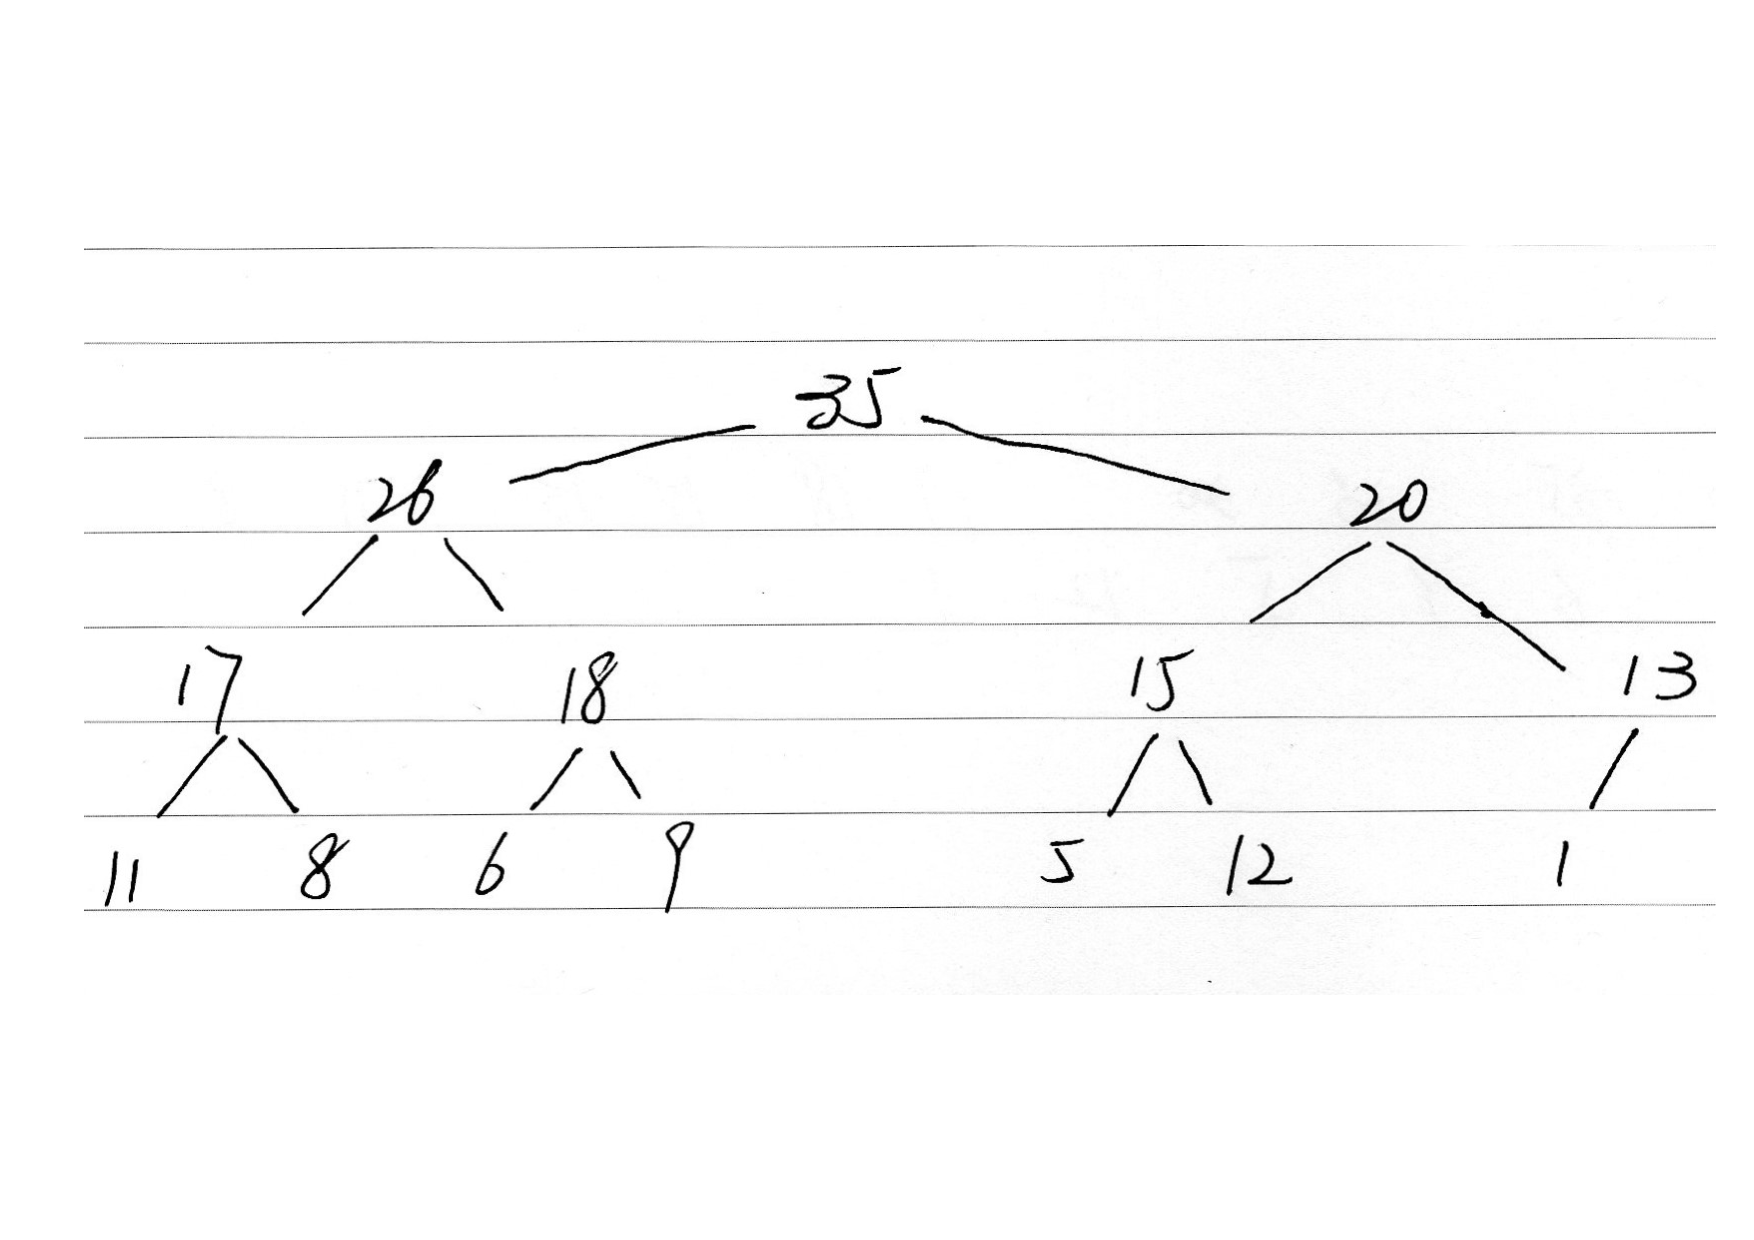
\includegraphics[width=\textwidth]{Pic/Part2_Prob1_Heap.pdf}
    \caption{Max Heap}
  \end{figure}
\section*{Problem 2}
\begin{lstlisting}[language = C++]
<template T>
class MedianHeap<T>{
    MaxHeap<T>* max_heap;
    MinHeap<T>* min_heap;
    T median;
}
<template T> 
const T 
  input_and_output_median
  (const T new_num, MedianHeap<T>* mh){
    if (new_num > mh->median) {
      mh->max_heap->push(new_num);
    } else {
      mh->min_heap->push(new_num);
    }
    if ((mh->min_heap->size()+mh->max_heap->size()) & 1==0){
    // Even number of inputs
      // Maintain the shape of two heaps to make sure that the 
      // difference in the # of elements doesn't exceed 2.
      // To be more specific, if one heap has 2 more element than 
      // the other, take the root away and give that to the other 
      // heap.
      if (mh->min_heap->size() > mh->max_heap->size()) {
          mh->max_heap->push(mh->min_heap->pop());
      } else {
          mh->min_heap->push(mh->max_heap->pop());
      }
      // With two heaps of equal size,take the smaller one as median.
      mh->median = mh->min_heap->root();
    } else {
    // Odd number of inputs
      // Whichever heap with (one) more elements should take the root 
      // as median.
      if (mh->min_heap->size() > mh->max_heap->size()){
          mh->median = mh->min_heap->root();
      } else {
          mh->median = mh->max_heap->root();
      }
    }
    return median_heap->median;
}
\end{lstlisting}
\section*{Problem 3}
  \subsection*{(a)}
    $$\begin{bmatrix}
       5 & 11 & 14 & 24 \\
      45 & 47 & 54 & 98 \\
      \infty & \infty & \infty & \infty \\
      \infty & \infty & \infty & \infty 
    \end{bmatrix}$$
  \subsection*{(b)(c)}
    \par \textbf{Lemma}: $$\forall i, j$$$$ Y[1, 1] < Y[i, j] < Y[m, n]$$
    \par \textbf{Proof}: 
      $$Y[1, 1] < Y[1, j] < Y[i, j] < Y[i, n] < Y[m, n]$$
    \par Thus, if $Y[1,1] = \infty$, then there will be no finite number left, such that the matrix if empty.
    \par If $Y[m, n] < \infty$, then there will be no $\infty$ in the matrix, such that the matrix is full.
  \subsubsection*{(d)}    
\begin{lstlisting}[language = C++]
#define inf 0xffff
class YoungTableau;
<template T>
void 
  YoungTableau<T>::insert(const T num){
    int i = 0, j = this->col-1;
    while !((i==this->row-1) && (j == this->col-1)){
      if (j == 0) {
        // We can directly add this number if this matrix is empty.
        // Or we can start a new line as long as it's larger than 
        // the last line's first element.
        if ((i == 0) || (num > this->table[i-1, 0])) {
          this->table[i,0] = num;
        } else {
        // Otherwise we can't add this number.
          stderr("No way of adding this number.")   
        }
        break;
      }
      // If we hadn't reach the head of the row:
      if (this->table[i,j-1] == inf){
        // more forward until the front is not inf,
        j--;
      } else {
        if (num > this->table[i, j-1]) {
          // add the number if suitable,
          this->table[i, j] = num;
        } else {
          // or goes to next line and try better luck.
          i ++;
        }
      }
    }
}
\end{lstlisting}
  \subsection*{(e)}
\begin{lstlisting}[language = C++]
<template T>
const T* 
  const YoungTableau<T>::sort(){
    auto temp_table = this->table;
    T* arr = (T) malloc(sizeof(T) * this->size());
    int len = 0;
    for (int s=0; s++; s<2*this->col-2){
      for (k=0; k<s; k++){
        int j;
        T* min
        for(int i=max(0, s-this->col); 
            i<min(s, this->col); 
            i++){
          j = s-i;
          if (temp_table[i,j] < *min) {
            min = &table[i,j];
          }
        }
        if (*min != inf) {
          arr[len] = *min;
          len ++;
        } else {
          break;
        }
      }
    }
    return arr;
}
\end{lstlisting}
\end{document}
